%how to cite
%\cite{Seow2011}
%how to add figure



\newpage
\section{Introduction}

\subsection{Obstacle Avoidance using RL and DL}
The navigation capability is a fundamental problem of mobile robots, which include unmanned vehicles, aerial vehicles, and ships. The general aim of navigation is to identify an optimal or sub-optimal path from a starting point to a target point in a Two-Dimensional (2D) or Three-Dimensional (3D) environment while avoiding obstacles. Delivery robots, warehouse automated guided vehicles, and indoor service robots require robust robot navigation systems in their dynamic environments. 
Adding autonomous navigation ability to robot platforms boosts their performance significantly since they can reach wherever they are needed on their own. This motivation has driven researchers to push the autonomous navigation technology to its limits.
Over the years, computers have evolved dramatically reducing the computational burden for mobile robot platforms. This has paved the road toward using more powerful methods like DL and reinforcement learning which have higher processing power requirements.
Inspired by interesting learning results achieved by RL, it has been extended to handle problems with continuous state and action spaces. This trend has been reinforced by borrowing ideas from DL giving birth to robust deep RL (DRL) methods capable of controlling robots with continuous and high dimensional states and action spaces. For example, Cheng et al.\cite{Cheng2022} applied DRL for path following and obstacle avoidance.



\subsection{DRL-based Navigation}

Mobile robots include unmanned vehicles, aerial vehicles, and ships that move in two or three dimensions. Their navigation involves searching for an optimal or sub-optimal path from the starting point to a target point while avoiding obstacles. To simplify this challenge, most researches have focused only on the navigation problem in 2D space.
The purpose of using a DRL algorithm in an autonomous navigation task is to find the optimal policy for guiding the robot to its target position through interaction with the environment. Many well-known DRL algorithms, such as DQN\cite{mnih2013}, DDPG\cite{lilli2015}, PPO\cite{schulman2017}, and their variants, have been extended to realize a DRL-based navigation system. These methods describe the navigation process as an MDP that uses sensor observation as the state with the goal of maximizing the expected revenue of the action. As mentioned above, DRL-based navigation has the advantages of being mapless and having a strong learning ability and low dependence on sensor accuracy. As RL is a trial- and-error learning technology, the physical training process inevitably leads to collisions of the robot with environmental obstacles, which is prohibited. Generally, the deep neural network is trained in a simulation environment before being deployed in a real robot for real-time navigation decision making.
DRL-based navigation has been used to replace or be integrated into the traditional navigation framework. Figure \ref{fig:DRLNavSys} shows the interaction process between the agent and environment of the DRL-based navigation system. The DRL agent replaces the localization and map building module as well as the local path planning module of the traditional navigation framework, moving toward the target point while avoiding static, dynamic, and simple structurally continuous obstacles. However, in an environment where structurally continuous obstacles are too complex, the agent may fall into a local trap. In this case, DRL requires additional global information provided by the traditional navigation technique.
 
\begin{figure}[h!]
	\centering
	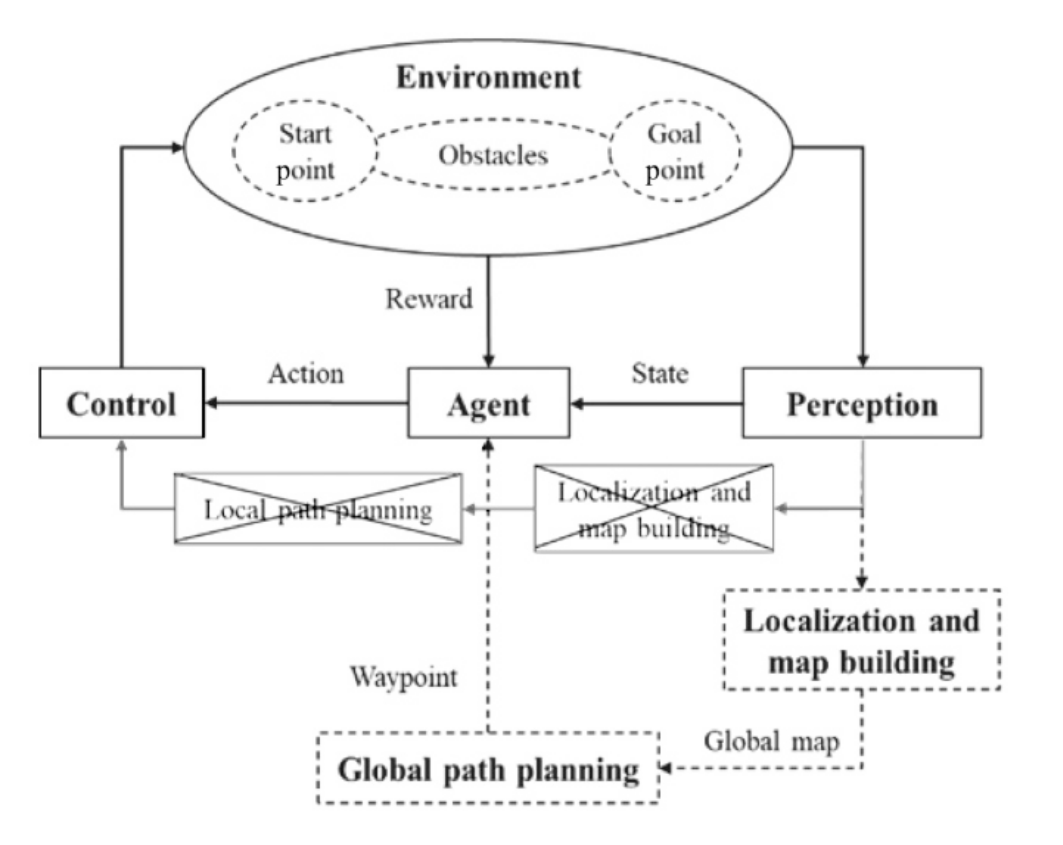
\includegraphics[width=0.8\linewidth]{figures/drl-based-nav.png}
	\caption{DRL-based Navigation System}
	\label{fig:DRLNavSys}
\end{figure}


